Queremos graficar los datos obtenidos en el experimento de la resistencia simple.
Nosotros sabemos que la relación entre el voltaje \( V \) y la corriente \( I \)
en un resistor es lineal y está dada por la ley de Ohm:
\[
V = I \cdot R
\]
donde \( R \) es la resistencia del resistor. Para graficar los datos, necesitamos
medir el voltaje y la corriente en el circuito y luego representar estos valores
en un gráfico de \( V \) versus \( I \). A partir de la pendiente de la línea obtenida en el gráfico,
podremos determinar el valor de la resistencia \( R \). Aproximacion lineal que será:

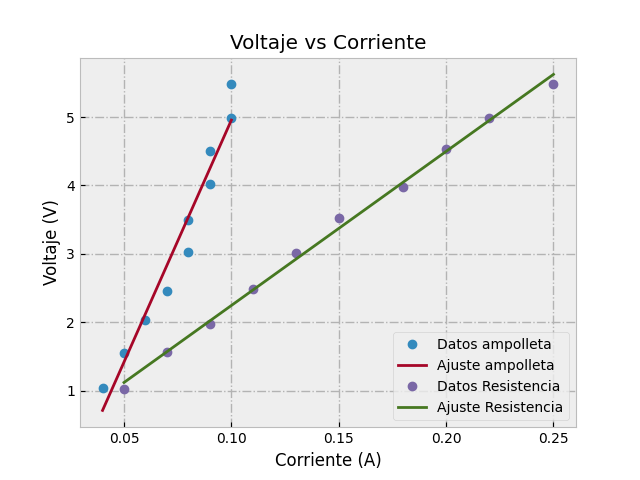
\includegraphics[width=0.7\textwidth]{ampolleta.png}